\section{Implementierung}

 	siehe Paper über EEXCESS
 \subsection{Verwendung von AngularJS für alle Komponenten des Plugins}
 Für die Implementierung von Jarvis wurde sich für AngularJS\footnote{\url{https://angularjs.org/}} entschieden. Das von Google entwickelte JavaScript MVC-Framework bietet einige Vorteile, die Webentwicklung im Allgemeinen und die Entwicklung dieser Extension erleichtern.

 AngularJS erlaubt es eigene Direktiven zu entwerfen. Direktiven beschreiben wie ein HTML Element dargestellt werden soll und wie es (z.B. auf Benutzerinteraktionen) reagieren soll \cite{jain2015angularjs}. Sie können dann wie HTML Tags oder Attribute genutzt werden. So wird eine hohe Wiederverwendbarkeit von Komponenten erzeugt. Genutzt wurde dieses Feature um eine Direktive zu entwickeln, mit der die Paragraphen der Webseite ``verpackt'' werden. Die neue Direktive enthält die Funktionen um eine Suchanfrage zu bauen und zu senden und die graphischen Elemente um die Resultate anzuzeigen. 

 Weiterhin befindet sich in den meisten Frameworks das Markup in einem Template. Dieses Template wird dann in HTML kompiliert und in das Document Object Model (DOM) geladen \cite{jain2015angularjs}. Das Markup der AngularJS Application befindet sich innerhalb des HTML-Dokuments. Dadurch ist es möglich, dass AngularJS das Markup erst auswertet, nachdem es in das DOM geladen wurde \cite{jain2015angularjs}. Von den Vorteilen die dadurch entstehen ist einer für die Entwicklung von Jarvis besonders nützlich: Da AngularJS die Seite erst nach dem Laden auswertet, ist es einfach, AngularJS Module in existierende Webseiten zu integrieren \cite{jain2015angularjs}. Mit Jarvis möchte genau das erreicht werden. Zu einer bestehenden Seite soll Funktionalität hinzugefügt werden. Zusammen mit JavaScript Injection kann man auf diese Weise innerhalb des Client-Browsers AngularJS Logik in eine beliebige Seite integrieren, ohne die eigentliche Implementierung der Seite zu verändern.

 Der Modul-basierte Aufbau von AngularJS Anwendungen gestattet außerdem eine leichte Erweiterbarkeit und Austauschbarkeit der Komponenten. Einzelne Dienste, wie bei Jarvis die Extrahierung der Schlüsselwörter oder die Kommunikation mit Europeana, sind in Module oder Services verpackt und können so einfach durch andere ersetzt werden. So kann man die Extension leicht auf andere Suchmaschinen umbauen oder andere Algorithmen zur Analyse der Paragraphen verwenden.

 Unabhängig von der Entwicklung von Jarvis bietet AngularJS einen weiteren großen Vorteil: Two way data-binding \cite{jain2015angularjs}. Im Gegensatz zu anderen Frameworks oder zu reinem JavaScript, wo man manuell jede Änderung des Models an die View propagieren muss und anderes herum, übernimmt AngularJS diese Aufgabe. Ändert sich das Model, wird automatisch das jeweilige DOM Element angepasst. Interagiert der User mit einem Element, werden Änderungen sofort an das dahinter stehende Model weitergeben. Das reduziert den benötigten Code und erlaubt eine schnelle und saubere Entwicklung von Anwendungen.

 \subsection{Architektur der Extension}
 Wie in Abbildung \ref{fig:architektur} zu sehen ist, ist Jarvis in vier AngularJS Module unterteilt:
 \begin{enumerate*}[label=\alph*\upshape)]
 	\item Jarvis für die Content-Skripte,
  	\item JarvisBG für die Background-Skripte,
 	\item JarvisPopup für die Browser-Action, und
 	\item JarvisSettings für die Options-Page.
 \end{enumerate*}
 Im folgenden Absatz beschreibt Jarvis das Modul der Content-Skripte und nicht die gesamte Extension.

 \begin{minipage}{\linewidth}
	\centering
	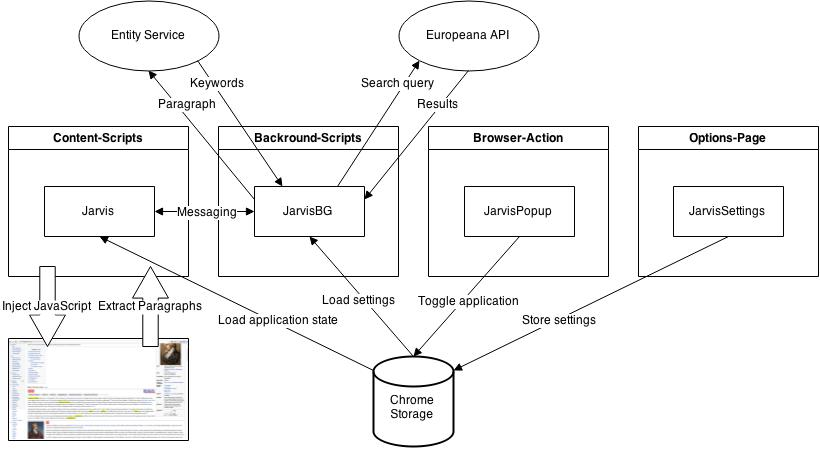
\includegraphics[width=\linewidth]{Bilder/architektur.jpg}
	\captionof{figure}{Kommunikation der AngularJS Komponenten untereinander}
	\label{fig:architektur}
 \end{minipage}
 
 Jarvis ist das Modul, welches in die jeweilige Webseite per JavaScript Injection eingefügt wird. Es extrahiert die Paragraphen aus dem Text und fügt die eigene Direktive in das DOM ein. Die extrahierten Paragraphen werden per Message Passing\footnote{\url{https://developer.chrome.com/extensions/messaging}} an die Background-Skripte weitergegeben. Diese sind zusammengefasst im Modul JarvisBG. 

 Dieses Modul ist zuständig für die Kommunikation mit den REST Endpunkten von Europeana und dem Keyword Service. Im Gegensatz zu Jarvis, welches für jeden offenen Browser-Tab eine eigene Instanz hat, existiert das JarvisBG Modul nur ein mal (wie auch JarvisPopup und JarvisSettings). Jarvis schickt Nachrichten mit dem Namen des angeforderten Services sowie einer Callback-Methode an JarvisBG. Dieses führt die Anfrage aus und übergibt die Ergebnisse der Callback-Methode. Diese sorgt dann dafür, dass die Ergebnisse im Frontend richtig angezeigt werden. 

 JarvisPopup ist das Modul des Popup-Fensters, welches nach klick auf das Icon der Extension rechts des Adressfeldes angezeigt wird. Über das Popup wird der Zustand der Extension im aktuellen Tab gesteuert. Der User kann hier entscheiden, ob das Programm in diesem Tab angezeigt wird oder nicht. Der Zustand wird dann im Chrome Storage\footnote{\url{https://developer.chrome.com/extensions/storage}} gespeichert. Die Wahl für die Speicherung der Anwendungsdaten viel auf den Chrome Storage, da er einige Vorteile gegenüber der localStorage API\footnote{\url{https://developer.mozilla.org/en-US/docs/Web/Guide/API/DOM/Storage\#localStorage}} bietet. Zum einen können die Content-Skripte direkt darauf zugreifen ohne einen Umweg über die Background-Skripte gehen zu müssen. Weiterhin erlaubt Chrome Storage eine automatische Synchronisierung der Inhalte. Dadurch wird Jarvis sofort benachrichtigt, sobald sich der Zustand der Applikation ändert.

 Der Nutzer hat die Möglichkeit, über die Options-Page\footnote{\url{https://developer.chrome.com/extensions/optionsV2}} die verwendeten Services zu konfigurieren. Das dafür zuständige Modul ist JarvisSettings. Es speichert die Einstellungen im Chrome Storage und JarvisBG passt die REST-Anfragen entsprechend an.

 \subsection{Paragraphen-Erkennung}
 \subsection{Paragraphen-Analyse}
  Improving Efficiancy and Accuracy in Multilingual Entity Extraction

 \subsection{Bau der GUIs}
		- > Darf den Benutzer nicht zu sehr ablenken
		- > Ergebnisse müssen in der Nähe ihrer „Quelle“ angezeigt werden (proximity compatibility pricinple)
		- > Benutzer muss klar zwischen Webseite und Augmentation unterscheiden können
		- > buntes, auffälliges Design
		- > Ramping interface: Mehr Benutzerinteraktionen führen zu mehr angezeigten Informationen (Erklärung der Stages) 


 Durch die Chips kann man später auch leicht IQE hinzufügen, zb relevance feedback
 \subsection{Einbindung der REST-Services}